\section{Background}
\subsection{Economic Rationale}
\begin{frame}{General Theory}
    \begin{itemize}
        \item The level of output is determined by the level of
              \textit{effective demand}.
              \begin{enumerate}
                  \item Effective demand is made volatile by the
                        presence of investment spending and
                        \textit{expectations} in the market.
              \end{enumerate}
        \item A change in aggregate industrial wide income $Y$ is
              impacted by a multiplier with investment
              and savings ($I$ and $S$).
              \begin{enumerate}
                  \item $\Delta I \rightarrow \Delta S$.
              \end{enumerate}
        \item The government can play a role in spurring \textit{effective
                  demand} using fiscal tools in the hydrogen market.
    \end{itemize}
    \footnotetext[1]{Keynes, John Maynard. 2021. \textit{The General Theory Of
            Employment, Interest And Money}. London: Palgrave Macmillan.}
\end{frame}
\begin{frame}{Taxation}
    \begin{itemize}
        \item The use of \textit{smart contracts} can `nudge' consumers of
              hydrogen to use cleaner hydrogen.
              \begin{enumerate}
                  \item A `carbon tax' enforced by a player in the system.
              \end{enumerate}
        \item Punishing non-clean sources of energy through smart contracts
              can accelerate the removal of negative externalities.
              \begin{enumerate}
                  \item Rapidly adjust to `cleaner' equilibria inside a market.
              \end{enumerate}
    \end{itemize}
\end{frame}
\subsection{Hydrogen Certificates}
\begin{frame}{Hydrogen Certificates}
    \begin{itemize}
        \item An approach for formally attesting the level of cleanness in
              a produced unit of hydrogen.
              \begin{enumerate}
                  \item Shared across the supply chain.
                  \item Can attest to standards related to Hydrogen
                        safety and quality.
              \end{enumerate}
        \item An agent in the blockchain can act as the certification body.
    \end{itemize}
\end{frame}
\subsection{Existing Work in Energy Domain}
\begin{frame}{Distributed Energy System}
    \begin{itemize}
        \item \textit{Li et al., (2019)} developed a blockchain
              architecture for the energy market using smart contracts
              with non-cooperative game theory.
    \end{itemize}
    \begin{figure}
        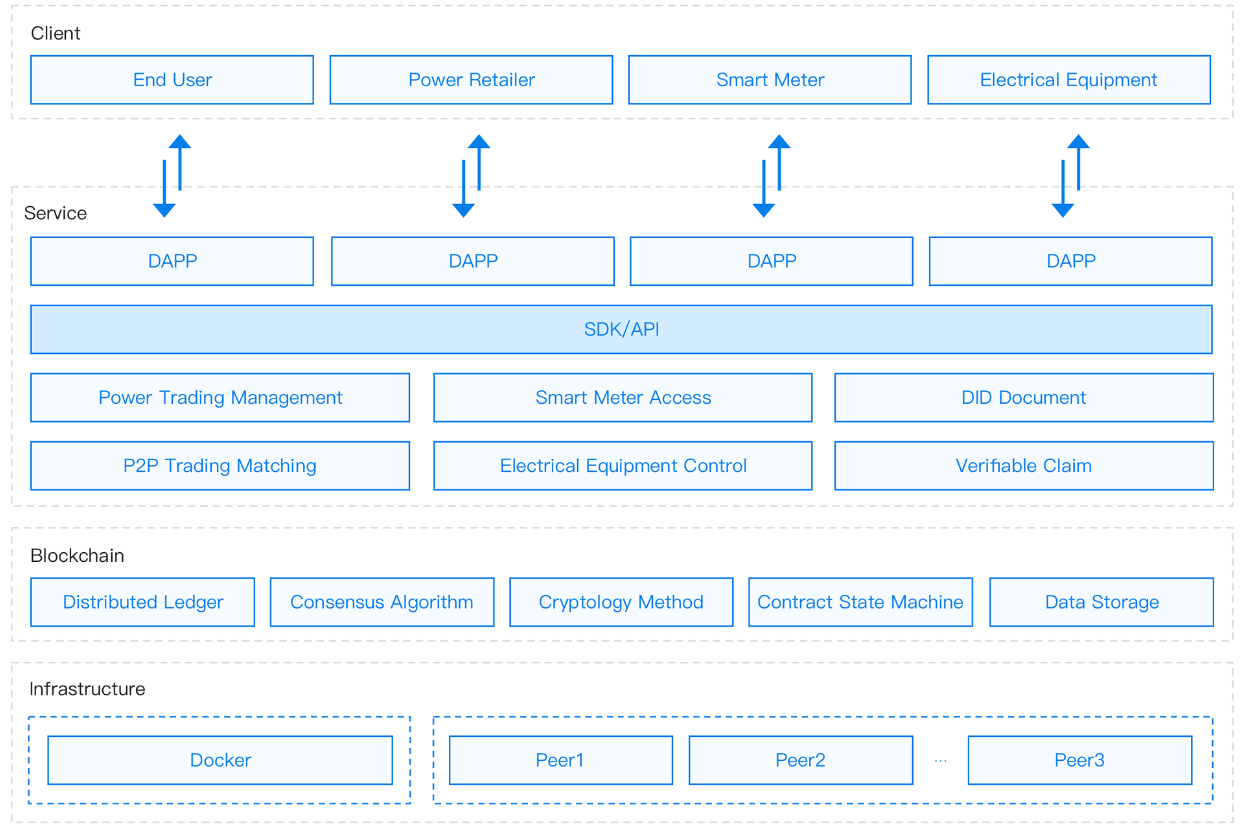
\includegraphics[height=0.5\textheight, width=\linewidth,
            keepaspectratio]{photos/blockenergy.png}
        \centering
    \end{figure}
    \footnotetext[1]{Li, Yinan, Wentao Yang, Ping He, Chang Chen,
        and Xiaonan Wang. 2019. "Design And Management Of A Distributed Hybrid
        Energy System Through Smart Contract And Blockchain".
        \textit{Applied Energy} 248:
        390-405. doi:10.1016/j.apenergy.2019.04.132.}
\end{frame}
\begin{frame}{CertifHy}
    \begin{itemize}
        \item A European certification scheme for clean hydrogen.
        \item 75,000 digital certificates issued.
        \item Software system.
        \item Allows for registration, issuing and transfer of certificates.
    \end{itemize}
    \footnotetext[1]{``Certifhy''. 2021. \textit{Certifhy.eu}.
        \url{https://www.certifhy.eu/}.}
\end{frame}
\subsection{Blockchain Patterns}
\begin{frame}{Patterns}
    \begin{itemize}
        \item Token template pattern
        \item Token registry pattern
        \item Escrow
    \end{itemize}
    \begin{figure}
        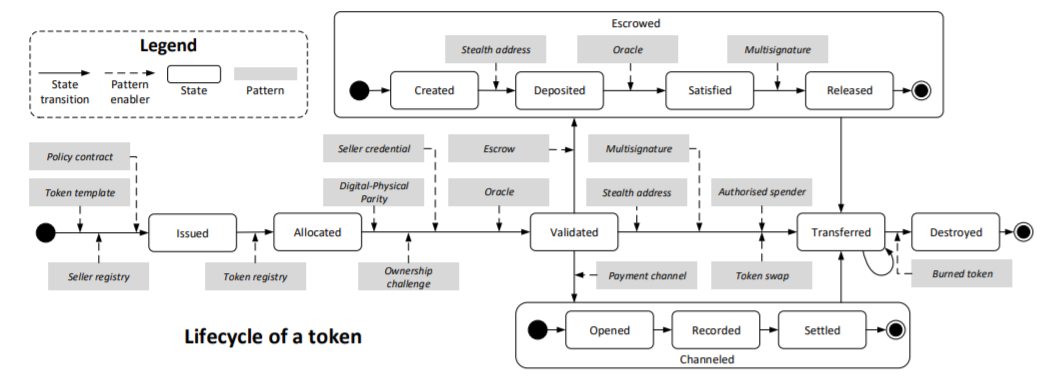
\includegraphics[height=0.5\textheight, width=\linewidth,
            keepaspectratio]{photos/token.png}
        \centering
    \end{figure}
    \footnotetext[1]{Lu, Qinghua, Xiwei Xu, Dilum Bandara, Shiping Chen,
        and Liming Zhu. 2021. \\
        ``Design Patterns For Blockchain-Based Payment Applications''.
        \textit{ACM}. doi:10.1145/1122445.1122456.\\}
\end{frame}
\subsection{Hyperledger Fabric}
\begin{frame}{Fabric}
    \begin{itemize}
        \item A modular and extensible open-source system for
              developing blockchain applications.
        \item Pluggable consensus algorithms.
        \item \textit{Chaincode} in general programming languages.
        \item Channels for enterprise confidentiality.
    \end{itemize}
    \begin{figure}
        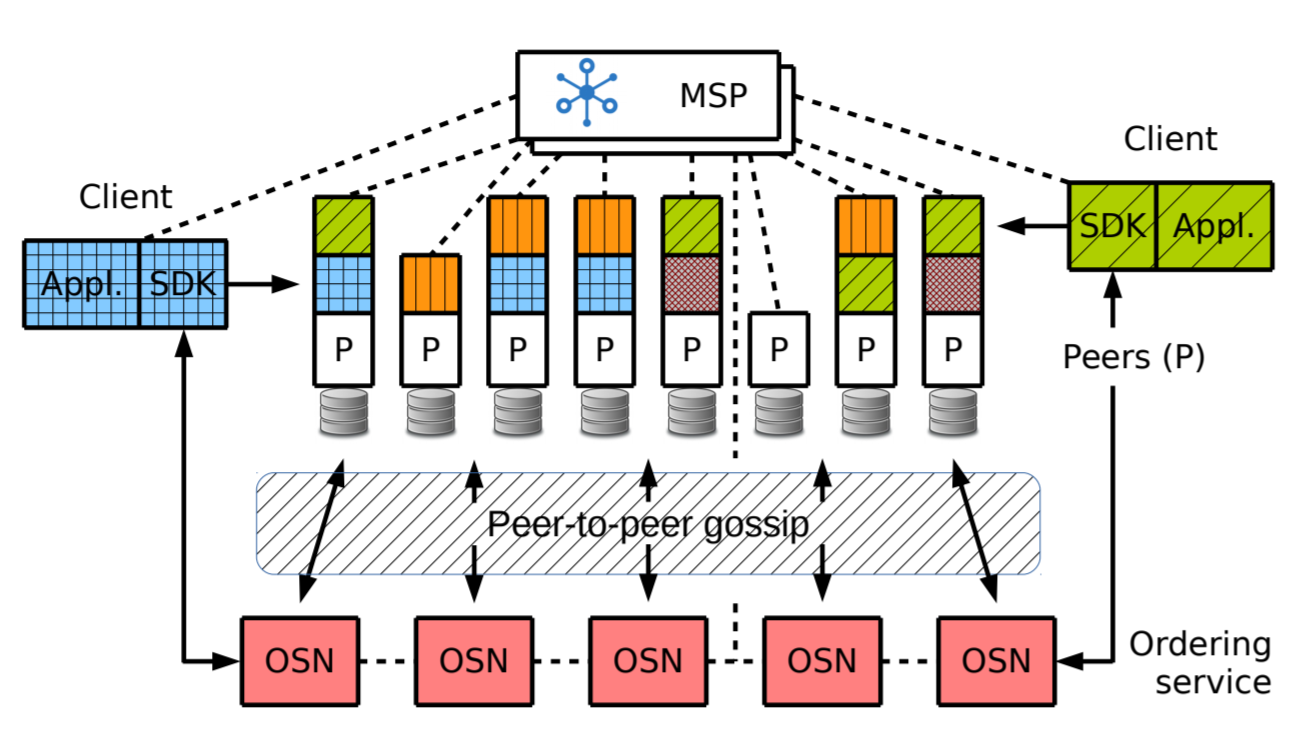
\includegraphics[height=0.4\textheight, width=\linewidth,
            keepaspectratio]{photos/fabric.png}
        \centering
    \end{figure}
    \footnotetext[1]{Androulaki, Eli, Artem Barger, Vita Bortnikov, Christian Cachin, et al.
        2018.
        ``Hyperledger Fabric: A Distributed Operating System For
        Permissioned Blockchains''.}
\end{frame}
\begin{frame}{Fabric Architecture}
    \begin{itemize}
        \item Novel \textit{execute-order-validate} architecture
              supporting high throughput transactions.
        \item Dedicated ordering nodes.
        \item Support for up to 3560 TPS (lab environment).
    \end{itemize}
    \begin{figure}
        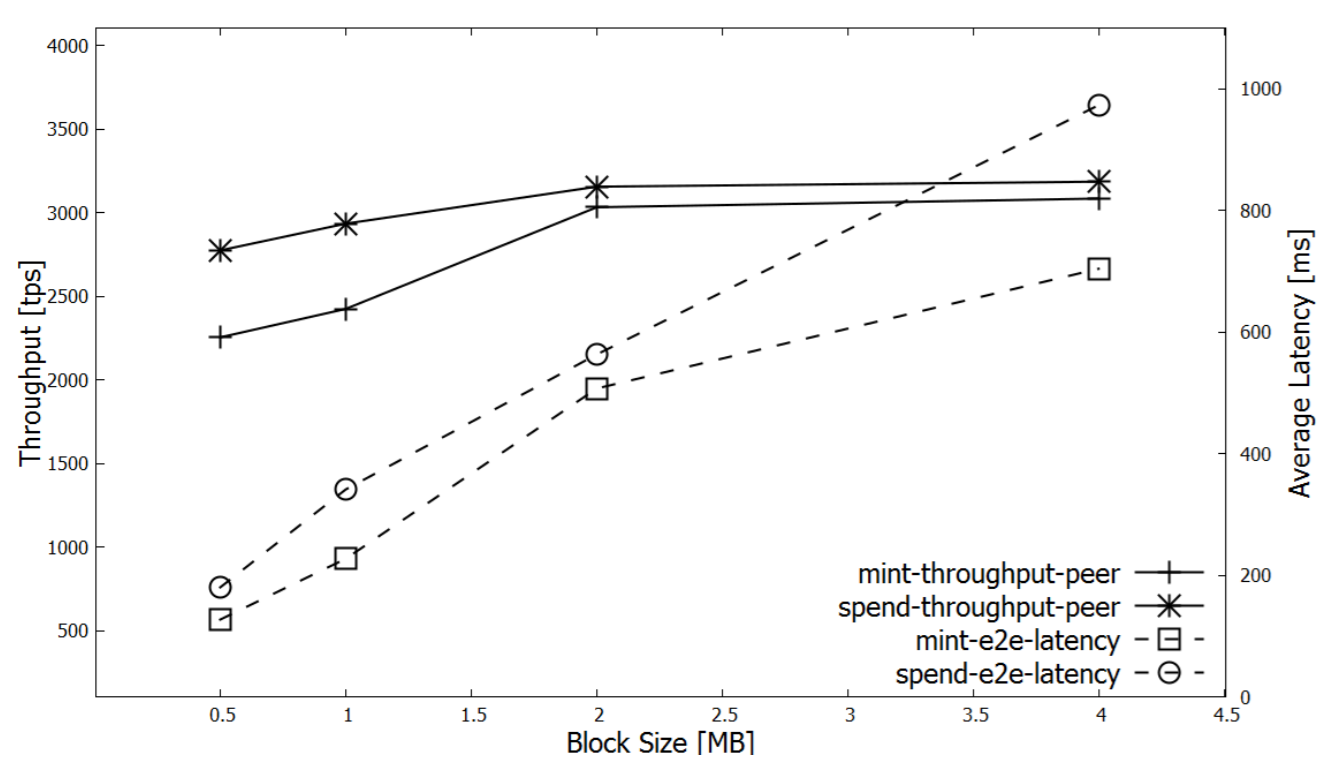
\includegraphics[height=0.4\textheight, width=\linewidth,
            keepaspectratio]{photos/tps.png}
        \centering
    \end{figure}
    \footnotetext[1]{Androulaki, Eli, Artem Barger, Vita Bortnikov, Christian Cachin, et al.
        2018.
        ``Hyperledger Fabric: A Distributed Operating System For
        Permissioned Blockchains''.}
\end{frame}
\subsection{Fabric Projects}
\begin{frame}{Fabric Projects}
    \begin{itemize}
        \item GoDirect Trade introducing trust into the supply chain for used
              aeroplane parts.
        \item OrgBook British Columbia helping small businesses find critical
              information about business partners.
        \item A permissioned blockchain as a `trust machine' for organisations.
    \end{itemize}
    \footnotetext[1]{
        ``Orgbook Case Study – Hyperledger''. 2021. \textit{Hyperledger}.
        \url{https://www.hyperledger.org/learn/publications/orgbook-case-study}.
    }
    \footnotetext[2]{
        `Case Study: Honeywell Aerospace Creates Online Parts Marketplace With
        Hyperledger Fabric'.
        2021. Blog. \textit{Case Studies}. Accessed April 14.
    }
\end{frame}
\subsection{Summary}
\begin{frame}{Summary}
    \begin{itemize}
        \item The government can use the blockchain to deliver trust and growth
              in hydrogen energy.
        \item Smart contracts can be applied for verification of hydrogen
              quality.
        \item Previous blockchain energy
              solutions rely on centralised parties
              or use the blockchain to act as an `auction house'.
    \end{itemize}
\end{frame}